\documentclass[10pt,a4paper]{article}

\usepackage[utf8]{inputenc}
\usepackage[dutch]{babel}
\usepackage{fancyhdr}
\usepackage{geometry}
\usepackage{graphicx}
\usepackage{tabularx}
\usepackage{wallpaper}
\usepackage{listings}
\usepackage{amsmath}
\usepackage{parskip}
\usepackage{gensymb}

\usepackage{xcolor, colortbl}
\definecolor{ugentblue}{HTML}{164A7C}
\definecolor{gray}{HTML}{AAAAAA}
\definecolor{lightgray}{HTML}{FAFAFA}
\definecolor{grayborder}{HTML}{CCCCCC}
\definecolor{commentgreen}{HTML}{009900}

% Tables
\def\arraystretch{1.35}
\renewcommand{\tabularxcolumn}[1]{>{\small}m{#1}}
\newcommand{\hcell}[1]{
	\cellcolor{ugentblue}\color{white}\textbf{#1}
}

\makeatletter
\renewcommand\thesubsection{\@arabic\c@section.\@arabic\c@subsection}
\makeatother{}

\usepackage[hypertexnames=false]{hyperref}
\usepackage[numbered, depth=3]{bookmark}

\renewcommand{\headrulewidth}{0pt}
\pagestyle{fancy}
\fancyhf{}

\interfootnotelinepenalty=0

% Listings
\lstset{
	backgroundcolor=\color{lightgray},
	basicstyle=\footnotesize,
	commentstyle=\color{commentgreen},
	frame=single,
	framesep=7pt,
	keywordstyle=\color{blue},
	language=Java,
	numbers=none,
	numbersep=5pt,
	numberstyle=\tiny\color{gray},
	rulecolor=\color{gray},
	stepnumber=1,
	stringstyle=\color{ugentblue},
	showspaces=false,
	showstringspaces=false
}

\begin{document}
	\begin{titlepage}
		%% Footer
		\thispagestyle{fancy}
		\fancyhf{}

		%% Page
		\hfill
		\begin{minipage}[t][0.9\textheight]{0.8\textwidth}
			\noindent
			
\includegraphics[width=55px]{ugent-blue.png} \\[-1em]
			\color{ugentblue}
			\makebox[0pt][l]{\rule{1.3\textwidth}{1pt}}
			\par
			\noindent
			\textbf{\textsf{Vage Databanken}} \textcolor{gray}{\textsf{Academiejaar 2014-2015}}
			\vfill
				\noindent
			{\huge \textsf{Project Vage Databanken}}
			\vskip\baselineskip
			\noindent
			\textsf{Groep 8 \\
				\textbf{Jasper D'haene} \\
				\textbf{Florian Dejonckheere}}
		\end{minipage}
	\end{titlepage}

	%%% PAGE STYLE %%%
	\nopagecolor
	\renewcommand{\footrulewidth}{0.4pt}
	\headheight 45pt
	\ULCornerWallPaper{1}{header.png}
	\fancyfoot[C]{\thepage}

	%%% DOCUMENT %%%
	\section{Generiek vaagregelsysteem}
		Beschrijving van het \texttt{FuzzySystem}. \\

		In het project werd gebruik gemaakt van de volgende extra libraries: de \href{https://commons.apache.org/proper/commons-math/}{Apache Commons Mathematics} library en de \href{https://code.google.com/p/json-simple/}{JSON.simple} library. De Apache Commons Math library voorziet een stabiele numerieke implementatie van verscheidene integratiemethoden. Omdat de integratieperformantie belangrijker is dan de precisie, werd gekozen voor de simpelste implementatie -- de \texttt{MidPointIntegrator} -- met een relatief kleine precisie.\\

		Alle parameters die de vorm van de lidmaatschapsfuncties bepalen zijn opgeslagen in de \texttt{resources} map, geserialiseerd in JSON. Deze bestanden worden ingelezen via de JSON.simple library en in het systeem ingevoerd aan de hand van de gegeven regels.\\

		Een probleem die al vroeg in de ontwikkeling voorkwam, betreft het onconditioneel limiteren van een aspect in de output. Stel dat er een conditie waarvoor onvoorwaardelijk moet gelden dat een outputvariabele nul is.

		\begin{lstlisting}
IF distanceFront IS minimal THEN acceleration IS none
		\end{lstlisting}

		Waarbij de lidmaatschapsfunctie van \texttt{acceleration IS none} een dunne clustering rond $0$ omvat. Deze regel kan zelfstandig niet worden uitgedrukt, aangezien het matchen van de conditie \texttt{distanceFront IS minimal} er niet met zekerheid voor zorgt dat het zwaartepunt van de resterende geaggregeerde lidmaatschapsfunctie op of onder $0$ terecht komt. Mogelijke oplossingen voor dit probleem zijn het combineren van elke regel die invloed heeft op \texttt{acceleration} met een \texttt{distanceFront IS minimal}-clausule, of een set equivalent, maar negatieve regels opstellen voor de positieve acceleratie-bepalende regels, zodat het zwaartepunt exact op $0$ valt. Beide oplossingen zijn omslachtig en onschaalbaar.\\

		Analoog vormt het maximum van een lidmaatschapsfunctie ook een probleem. Zoals het vaag regelsysteem gedefinieerd is, is het onmogelijk om de maximumwaarde te behalen van de lidmaatschapsfunctie van een outputvariabele. Als de \texttt{Consequence} van de regel niet gelimiteerd wordt ($\texttt{limit} = 1$) en de regel dus volkomen van kracht is, zal de outputvariabele uiteindelijk het zwaartepunt van de lidmaatschapsfunctie zijn. Dit zal zelden de maximumwaarde zijn, maar meer frequent ongeveer in het midden tussen de begin- en de eindparameter ($\alpha$ en $\beta$ bij trapezo\"idale functies).\\

		Het systeem -- omvat in de \texttt{fuzzy/FuzzySystem} klasse -- wordt vooreerst leeg ge\"instantieerd, en daarna pas worden de regels opgegeven. Deze regels zijn intern opgeslagen in een \texttt{ArrayList}, waarover er ge\"itereerd wordt bij evaluatie. Deze regels hoeven slechts \'e\'enmaal ingevoerd te worden -- in de constructor van de controller (in casu zorgt de \texttt{BaseController} hiervoor).\\

		Daarnaast heeft het systeem ook een nood aan inputvariabelen en -waarden. Deze worden elke frame in de \texttt{getFrameControl()} methode ingevoerd. Intern worden de variabelen en hun bijbehorende waarden opgeslagen in een \texttt{HashMap}, gesorteerd op de naam van de variabele. Later kan dan de geaggregeerde lidmaatschapsfunctie bepaald worden uit een entry in de map. Vervolgens wordt het volledige systeem ge\"evalueerd aan de hand van de \texttt{evaluate()} methode.\\

		Hoewel het opgegeven controlesysteem natively gebruik maakt van het \texttt{float} datatype, werd de keuze gemaakt om met \texttt{double} te werken, voornamelijk omdat de Apache Commons Math library als in- en outputtype \texttt{double} heeft.

	\section{Controllers}
		\subsection{SafeController}
			\texttt{SafeController} legt de focus op het zo veilig mogelijk bereiken van de finish. De grootste limiterende factor in deze controller is dan ook de snelheid. Door het ontwerp van het systeem wordt de snelheid gelimiteerd tot ongeveer 91 km/h. Als bijkomende constraints is er ook een minimumsnelheid opgelegd, alsook een remmende werking als de auto achteruit rijdt (bijvoorbeeld na een frontale botsing).

			De besturing van de wagen wordt geregeld door een set van regels die geleidelijk draaien onder invloed van de ligging van de wagen op het parcours. Die ligging wordt door de volgende formule berekend.

			\begin{equation}
	ratio = \frac{sensor_{left}}{sensor_{right}}
			\end{equation}

			Vervolgens wordt er bijgestuurd afhankelijk van de proportie. Deze methode heeft het voordeel ten opzichte van een simpele plaatsbepaling ($sensor_{left} - sensor_{right}$) dat de breedte van de weg minder invloed heeft op de koerscorrectie.\\
			De output van de functie (de \texttt{Consequence}) heeft als lidmaatschapsfunctie een S-curve. Op deze manier zal een kleine afwijking ($ratio \approx 1$) zeer weinig invloed hebben, die stijgt naar mate $ratio$ afwijkt van $1$. Er werd bewust voor gekozen de outputvariabele \texttt{steering} binnen het domein niet te hoog te laten worden, zodat er zich minder of geen bruuske bewegingen voordoen.\\

			Merk ook op dat \texttt{SafeController} de minst geavanceerde controller in de reeks is. Hij wordt als basis gebruikt voor \texttt{SpeedController} en \texttt{RalyController}, en er zijn zodoende ook situaties die minder goed behandeld worden door \texttt{SafeController}.\\

		\subsection{SpeedController}
			\texttt{SpeedController} zal trachten zo snel mogelijk de finish te bereiken. Hierbij wordt gebruik gemaakt van een uitgebreide versie van de snelheidsregels van \texttt{SafeController}. De granulariteit van deze regels is groter: er zijn meer regels vereist om de wagen een gecontroleerde snelheid mee te geven. Ook het remmen schaalt mee, aangezien er bij een groter aantal regels over een component ook een grotere controle over het complementaire aspect gevraagd wordt.\\

			Het koerscorrectie-algoritme uit \texttt{SafeController} werd ook aangepast. Bij lagere snelheden (onder 100 km/h) wordt het systeem uit \texttt{SafeController} gebruikt -- die geeft een distributie van ongeveer $\pm 0.17$ tot $\pm 0.44$ -- maar bij hogere snelheden kan een minder precieze of grote beweging catastrofale gevolgen hebben. Daarom ligt bij hogere snelheden de effectieve drempel hoger, en zijn de bewegingen preciezer.\\

			Ter slippreventie werd in de eerste instantie een \textit{countersteering}-systeem ontwikkeld, maar later bleek dat door het aanpassen van de gevoeligheid ten opzichte van snelheid van de \textit{steering} regels dit niet meer nodig bleek. Er werd later uitgebreid op het \textit{countersteering} in \texttt{RallyController}. Dit is een maatregel voor worst-case scenarios en in de re\"ele wereld zou dit systeem nooit de bovenhand kunnen krijgen.\\

		\subsection{RallyController}
			\texttt{RallyController} breidt op zijn beurt uit op \texttt{SpeedController}. In \texttt{RallyController} wordt de nadruk gelegd op het \textit{driften}. Dit fenomeen kan men aansturen door een bocht te benaderen via \textit{oversteer}, waardoor de auto begint te slippen en er tegengestuurd moet worden om alsnog de bocht correct door te gaan. Deze aanpak is echter eerder theoretisch dan praktisch, omwille van de irregulariteiten in de parcours -- en in de re\"ele wereld -- die ervoor zorgen dat er af en toe net voor een bocht een kleine uitdieping is in de wanden van de weg. Dit wordt door de sensoren echter al als een meetbaar verschil tussen de linker- en rechtersensor bemerkt waardoor de auto uiteindelijk de verkeerde richting op rijdt. De parameters van de regels tweaken kan hier echter geen levensvatbare oplossing voor bieden. Bovendien is een werkende combinatie van remmen en \textit{oversteer} om de auto horizontaal te krijgen praktisch te complex, mede dankzij het feit dat de maximale \textit{steering} en remcapaciteit niet bereikt kan worden.\\

			Door deze theoretische en praktische afwegingen werd er voor een andere aanpak geopteerd. In plaats van opzettelijk de auto te doen slippen door een bocht in \textit{oversteer} te benaderen, worden de bochten nu aan hogere snelheid genomen. Door het draaien aan snelheden rond de 120-130 km/h zal de auto hoe dan ook beginnen slippen, waarna er enkel nog tegengestuurd hoeft te worden om de auto terug onder controle te krijgen. Het \textit{driften} kan gedetecteerd worden door de combinatie van laterale snelheid en het verlies van grip of \texttt{friction} op de banden. Als de auto eenmaal aan het \textit{driften} is zal de laterale snelheid de richting en snelheid aanduiden -- hoe sterk er uiteindelijk moet tegengestuurd worden. Deze aanpak heeft als voordeel dat ze onafhankelijk is van de positie op de weg of het verdere parcours. De auto zal tegensturen zodoende hij weer in rechte lijn zijn traject kan verder zetten, ongeacht wat de linker- en rechtersensor al dan niet dicteren.\\

	\section{Performantie}
		\subsection{Keuze t-norm en t-conorm}
			%% Is de keuze van t-norm en t-conorm belangrijk voor de prestatie (i.e. de gemiddelde snelheid) van de wagen?
			Het verschil tussen het gebruik van de diverse t-normen en t-conormen is verbazend klein. Een kleine test levert op dat het relatieve verschil tussen berekeningen met verschillende t-normen typisch minder dan 2-3\% betreft. Uiteindelijk laat dit zich praktisch niet opmeten in de prestatie van de controllers. Dit is te wijten aan de definitie van de gebruikte lidmaatschapsfuncties voor de premisses in de regels. Deze worden voornamelijk bepaald door trapezo\"idale pi-functies met grenzen die relatief dicht bij elkaar liggen. Hierdoor komt de situatie $\mu = 0.0$ of $\mu = 1.0$ meer voor. Als \'e\'en van de parameters van zo'n conjunctie of disjunctie $1.0$ of $0.0$ is, dan is de uitvoer van elke t-norm of t-conorm gelijk.\\

		\subsection{Robuustheid regelsysteem}
			%% Hoe robuust is uw regelsysteem voor verschillende races? Is de gemiddelde snelheid ongeveer dezelfde als u de wagen verschillende keren laat racen op een welbepaald parcours?
			\texttt{SafeController} wordt inherent gelimiteerd op snelheid, en daar kan ook effectief geobserveerd worden dat zowel de gemiddelde snelheid en de pieksnelheid dicht bij elkaar liggen. Dit fenomeen doet zich voor op alle parcours, omdat er vrij continu voldaan wordt aan de \texttt{distanceHigh}, terwijl \texttt{distanceLow} (en dus \texttt{brakeHigh}) minder dominant is. Uit dit feit volgt dan ook dat meerdere ritten met deze controller dan ook praktisch dezelfde effectieve gemiddelde en topsnelheid heeft.\\

			Bij \texttt{SpeedController} varieert de snelheid iets meer, omdat de grenzen die de afstand bepalen wat gevoeliger zijn. Op rechte stukken zal de controller proberen een zo groot mogelijke snelheid te halen (binnen het vermogen), terwijl hij bij obstakels al snel zal remmen en corrigeren. Binnen verschillende ritten van deze controller is de performantie nagenoeg gelijk.\\

			De \texttt{RallyController} is iets minder robuust. Daar de sensoren die het \textit{driften} detecteren zeer gevoelig zijn afgesteld kan het voorkomen dat de kleinste verandering in condities catastrofale gevolgen kan veroorzaken. Het tegensturen in een bocht gebeurt meestal ook zeer dicht in de nabijheid van een muur, dus een kleine verandering in hoe sterk de auto tegenstuurt kan een botsing met de muur veroorzaken. Na het uitvoerig testen en bijstellen van deze parameters gebeurt dit nog zelden op de gegeven parcours. Deze situaties kunnen uiteraard niet geheel uitgesloten worden volgens het nondeterminisme van de game-engine.\\

		\subsection{Minder performante parcours}
			%% Zijn er parcours waar uw controller minder goed presteert? Hoe komt dit?
			Sommige parcours -- zoals Spa Francorchamps en Silverstone -- hebben een bepaalde structuur die verraderlijke metingen kunnen geven. Scherpe bochten kunnen aanleiding geven tot foutieve metingen door de vooruitkijkende sensoren die voor de correcte sturing zorgen. In zo'n scherpe bocht kan het voorkomen dat de sensoren de fysieke bocht niet (voldoende) opmerken, en onmiddelijk een meting geven voor de wand tegenover de bocht. Hierdoor stijgt de $ratio$, maar niet voldoende om de wagen te corrigeren in de bocht. Dit effect wordt versterkt door grote snelheden.

			\begin{figure}[h]
				\centering
				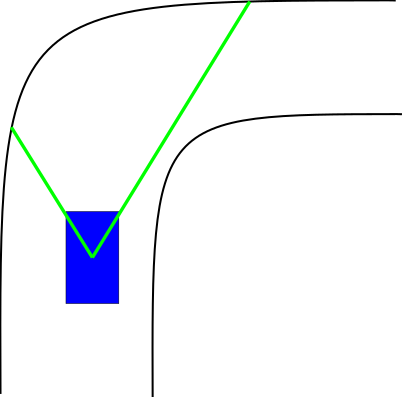
\includegraphics[width=5cm]{sensors-corner.png}
				\caption{Foutieve meting bij scherpe bochten}
				\label{fig:sensors-corner}
			\end{figure}

			Op zich zou dit probleem verholpen kunnen worden door de hoek van de sensoren continu adaptief aan te passen -- zodat een scherpe bocht toch opgemerkt wordt -- ware het niet dat de outputvariabelen van een enkele iteratie geen (meetbare) invloed hebben op de volgende iteratie. Opnieuw kan dit probleem suboptimaal opgelost worden door het intelligent gebruik maken van \textit{dampening}, waarbij beslist wordt of de output van de huidige iteratie authoritatief wordt doorgevoerd, of dat de vorige iteratie er invloed op hebben. Een goede optimalisatie voor dit karakter is een lokale \textit{cache} van sensorwaarden, zodat bepaalde probleempatronen en obstakels gedetecteerd kunnen worden. Dit systeem valt echter niet in de scope van dit project en wordt dus ook enkel als gedachte-experiment aangehaald.\\

			Uiteindelijk werd gekozen om een vaste sensorhoek -- $scanAngle = 0.9 = 30 \degree$ -- te hanteren, bepaald uit empirische experimenten op verschillende parcours met verschillende controllers.

			Het meest complexe parcours blijkt Spa Francorchamps te zijn. Dit parcours heeft even na de start een schijnbare bocht naar links die gevolgd wordt door een scherpe bocht naar rechts. Omdat de \texttt{frontSensor} echter het einde van de fysieke bocht naar rechts detecteert zal er door zowel de \texttt{SpeedController} als de \texttt{RallyController} een te hoge versnelling opgedragen worden. Eenmaal aangekomen aan de onverwachte bocht zal de hoge snelheid en plotse aanpassing in $ratio$ bij beide controllers zorgen voor een te bruuske koerscorrectie wat in de meeste instanties zal resulteren in een niet recupereerbare frontale botsing. Gezien het feit dat de controllers algemeen ontworpen werden was het niet mogelijk om voor deze specifieke (en unieke) situatie extra regels te voorzien die geen ongewenste effecten zouden veroorzaken op de overige parcours. Dit zou echter opgelost kunnen worden in een controller specifiek ontworpen voor dit parcours waar er geen stuuraanpassing gebeurt als de $ratio$ een bepaalde grens overschrijdt.\\

			Verbazingwekkend was het geografisch minst complexe parcour -- de Texas Speedway -- ook een van de lastigere parcours. Dit circuit bezit net als Spa Francorchamps een bepaalde situatie die het moeilijk maakt voor algemeen ontworpen controllers. Dit circuit is namelijk zeer breed en lang, waardoor een hoge snelheid dominant is bij de \texttt{SpeedController}. Na deze uitgebreide stroken volgen echter zeer bruuske bochten waardoor er niet voldoende geremd wordt en de auto bij de te scherpe draai begint te tollen. Dit kan in sommige situaties gunstig uitdraaien waarna de auto gewoon verder rijdt maar dit is zeker niet de norm. Als de snellere controllers aangepast zouden worden aan dit parcour zou dit echter resulteren in suboptimale tot zelfs teleurstellende prestaties op complexere parcours als Silverstone of Interlagos.\\

		\subsection{Veiligheid}
			%% Hoe veilig is uw wagen, i.e. hoe dikwijls crasht uw wagen?
			In dit model bestaat het concept \textit{veiligheid} enkel uit het contact met de wand, waardoor de \texttt{collisionSum} omhoog gaat. Het doel is uiteraard om de finish te bereiken met een zo laag mogelijke \texttt{collisionSum}.

			\texttt{SafeController} is ontworpen om zo veilig mogelijk de finish te bereiken. Door een gecontroleerd gebruik van de snelheid, lukt dit op de meeste parcours. Enkel op het Spa Francorchamps-parcours kan \texttt{SafeController} de laatste scherpe bocht van ongeveer $32 \degree$ net v\'o\'or de finish niet halen.\\

			De \texttt{SpeedController} zal hogere snelheden behalen maar zal geen onnodige risico's nemen in bochten door op tijd de rem in werking te stellen. Dit zou ook niet mogen aangezien deze controller maar uitgerust is met minimale koers-correctie in geval van slippen. Dit komt echter nagenoeg nooit voor - tenzij op het Texas parcours zoals eerder aangegeven - waardoor deze controller kan gezien worden als voldoende veilig.\\

			Zoals eerder aangegeven tijdens het bespreken van de robuustheid van de \texttt{RallyController} is deze controller minder veilig. Het is mogelijk dat deze controller tegen de muur rijdt, maar dit is meestal een zijwaartse collisie, waardoor de auto verder kan rijden. In uitzonderlijke gevallen zal er echter een frontale botsing plaatsvinden, wat de potenti\"ele onveiligheid van deze controller enkel bevestigt.\\

		\subsection{Exacte controller}
			%% Wat zijn de verschillen met een exacte controller (beter/slechter)?
			Een exacte controller reageert volgens welbepaalde scherpe grenzen op de input. Het grote verschil met deze systemen is dat er van een graduele aanpak geen sprake is. Bij een vaag regelsysteem kan de granulariteit van de response aangepast worden volgens constanten of andere (input-) parameters. Er kunnen meerdere regels zijn die betrekking hebben op \'e\'en aspect, en die dus elk tot op een bepaalde mate invloed hebben op de uitkomst van het systeem. \\

			Beschouw het volgende systeem met als output \texttt{acceleration}: Als er zich geen obstakels bevinden voor de auto, kan hij versnellen. Maar de versnelling moet gematigd zijn als de auto aan het driften is (dus als de laterale snelheid verschillend is van 0).
			Dit kan eenvoudig gemodelleerd worden door de volgende regels.

			\begin{lstlisting}
IF (distanceFront IS SMALL) THEN acceleration IS high
IF (lateralVelocity IS NOT ZERO) THEN acceleration IS low
			\end{lstlisting}

			Door het combineren van deze regels wordt in een drift rekening gehouden met zowel \texttt{acceleration IS high} en \texttt{acceleration IS low}, waardoor een gebalanceerd equilibrium uiteindelijk gekozen wordt als \texttt{acceleration}.
			Indien men dit in een exacte controller wil implementeren, moeten de twee regels gemultiplexd worden in \'e\'en formule. Dit kan bijvoorbeeld als volgt gebeuren.

			\begin{lstlisting}
int factor = 1;
if (lateralVelocity > 0)
	factor = 0.5;

return (1400 * (distanceFront / 200) * factor);
			\end{lstlisting}

			Deze formule bevat significant meer complexiteit en is ook sensitiever dan een vaagregelsysteem. Ook als er (foutieve) waarden optreden die buiten het definitiegebied vallen, kan de output een ongewenste waarde aannemen. Vage regelsystemen hebben hiertegen een intrinsieke bescherming, aangezien $\mu = 0$ buiten het definitiegebied van de lidmaatschapsfunctie.

		\section*{Eindopmerkingen}
			Het opgegeven systeem is inherent moeilijk te debuggen. De auto start altijd op dezelfde plaats, wat het lastig maakt om bugs in een later deel van het parcours te identificeren en corrigeren. Ook een vorm van temporele controle ontbreekt, waardoor bugtracking een passieve en tijdsintensieve activiteit wordt. Het gebrek aan sensoren maakt het detecteren van een catastrofale fout nagenoeg onmogelijk. Als de auto crasht met een voldoende grote snelheid, kan de physics engine ervoor zorgen dat deze uiteindelijk omgekeerd terechtkomt. De controllers zijn zich niet bewust van deze ontwikkeling, en rijden na\"ief verder -- de verkeerde richting op.\\

			Ook is er een schijn van non-determinisme aanwezig, waardoor volgens het \href{https://en.wikipedia.org/wiki/Butterfly_effect}{butterfly-effect} elke beweging van bijvoorbeeld het scherm (out-of-focus gaan) of camera aanpassing, tot een compleet ander eindresultaat leidt. Daardoor is het ontwikkelen van een algemene controller -- die op alle parcours, in alle races, dezelfde acceptabele performantie heeft -- moeilijk tot zelfs onmogelijk.\\

			Uiteindelijk kunnen de controllers voor elk parcours geoptimaliseerd worden, omdat elk parcours zijn eigen karakteristieken bezit. De Texas Speedway bijvoorbeeld, heeft er baat bij dat er zeer snel gereden wordt, en dat slechts kleine koerscorrecties uitgevoerd worden. Remmen hoeft in principe niet. Omdat in dit project de nadruk wordt gelegd op het ontwikkelen van een algemene controller, wordt dit niet in detail uitgewerkt.\\

			Hoewel een vaag regelsysteem uitstekend geschikt is voor het ontwerpen van praktische toepassingen zoals soft controllers, bevat het opgegeven systeem te weinig invoerdata om een acceptabel resultaat te produceren. Bepaalde situaties kunnen niet gemodelleerd en dus ook niet gedetecteerd en voorkomen worden. Voor bepaalde situaties -- zoals het gebruik van een adaptieve \texttt{scanAngle} -- kan een exact regelsysteem een goede oplossing bieden. De optimale oplossing is dan ook de gulden middenweg: een hybride combinatie van een vaag en een exact regelsysteem die ervoor zorgt dat de controller een gevarieerd gedrag bezit, en die intelligent rekening houdt met de omgeving en de in- en outputvariabelen.

\end{document}
